\documentclass[a4paper,12pt]{scrreprt}
    %% Used for changing geometry of the page
    %% Cover page text cannot overlay cover sketching/style 
    %% https://ctan.org/pkg/geometry?lang=en
\usepackage{geometry}
    %% Changes language of some packages protocols
    %% e.g., when captioning images: Figure 1. -> Figura 1.
    %% https://ctan.org/pkg/babel?lang=en
\usepackage[portuguese]{babel}
    %% Used for special fonts
    %% Cannot be compiled with pdflatex
    %% https://ctan.org/pkg/fontspec?lang=en
\usepackage{fontspec}
    %% Arial FONT
    \setmainfont{Arial}
\usepackage{subfiles}
    %% More colors and color options
    %% https://ctan.org/pkg/xcolor?lang=en
    %% https://ctan.org/pkg/colortbl?lang=en
\usepackage{xcolor,colortbl}
    %% More tabular options, like dashed/dotted lines
    %% https://ctan.org/pkg/arydshln?lang=en
\usepackage{arydshln}
    %% List of acronyms
    %% https://ctan.org/pkg/nomencl?lang=en
\usepackage[intoc]{nomencl}
    %% Must be called to init nomencl environment  
    \makenomenclature
    %% More images options/settings
    %% https://ctan.org/pkg/graphicx?lang=en
\usepackage{graphics}
    %% Defining subdirectories to image path enviornment
    %% \graphicspath{{sub1}{sub2}...{subN}}
    \graphicspath{{images}}
    
    %% used to handle cross-referencing commands in LaTeX to produce hypertext links in the document
    %% https://ctan.org/pkg/hyperref?lang=en
\usepackage{hyperref}
    %% math environments
    %% https://ctan.org/pkg/amsmath?lang=en

    %% settings
    \hypersetup{
        colorlinks,
        citecolor=black,
        filecolor=black,
        linkcolor=black,
        urlcolor=black
    }

\usepackage{amsmath}
    %% Defining backgrouns, used to make the cover
    %% https://ctan.org/pkg/background?lang=en
\usepackage[some]{background}
    %% Used to make drawings or complex graphics
    %% http://pgf.sourceforge.net/pgf_CVS.pdf
\usepackage{tikz}
    %% Tikz library to point operations ((x1,y1) + (x2,y2))
    \usetikzlibrary{calc}

%% Defining sfdefault font and default font for document
\renewcommand{\familydefault}{\sfdefault}


%% Costume made cover 
%% From there you can use \makecover command to build the cover
%% Blue cover color
\definecolor{titlepagecolor}{RGB}{54,95,145}

%==========================================================================
% COLORED BAR ON THE LEFT SIDE
%==========================================================================

\backgroundsetup{
    scale=1,
    angle=0,
    opacity=1,
    contents={
            \begin{tikzpicture}[remember picture,overlay]
                \path [fill=titlepagecolor]
                (current page.north west) -- ($(current page.north west) + (5,0)$)
                -- ($(current page.south west) + (5,0)$)-- (current page.south west);
                \node[color=white] at ($(current page.south west) + (3,4)$) {\bfseries {\fontsize{50}{60} \textsf{DSS}}};
                %\node[color=titlepagecolor] at ($(current page.south west) + (5.8,4)$) {\bfseries {\fontsize{120}{60} \textsf{4}}};
            \end{tikzpicture}
        }
}

%==========================================================================
% TITLE PAGE INFO
%==========================================================================

%% Changes values in this field to show information in the cover and back cover about your team/project


%% TITLE
\title{Sistema de apoio a departamento técnico}

%% AUTHORS
\author{
    \begin{tabular} { c c }
        
\includegraphics[scale=0.2]{author/marco.jpg} & 
\includegraphics[scale=0.2]{author/marco.jpg} \\
        62608 - Marco Sousa                           & 93198 - Mariana Marques                       \\
        %\hline                                                                                        \\
        
\includegraphics[scale=0.2]{author/marco.jpg} & 
\includegraphics[scale=0.2]{author/miguel.jpg} \\
        93271 - José Malheiro                         & 94269 - Miguel Fernandes
    \end{tabular}
}

%% Date

\date{\today}

%% Course
\newcommand{\Course}{Licenciatura em Engenharia Informática}

%% Department
\newcommand{\Department}{Escola de Engenharia}

%% UniName
\newcommand{\UniName}{Universidade do Minho}

\newcommand{\UcName}{Desenvolvimento de Sistemas de Software}

\newcommand{\GroupId}{Grupo 31}

%% UniPic
\newcommand{\UniPic}{
\includegraphics[scale=0.09]{uminho.png}}

%% University 
\newcommand{\University}{
    \begin{flushleft}
        \UniPic
    \end{flushleft}
    \textcolor{gray}{\small\textbf{\textsf{\UniName}}}\par
    \textcolor{gray!80!white}{\small{\textsf{\Department}}}\par
    \textcolor{gray!70!white}{\small{\textsf{\Course}}}
}

%% UC
\newcommand{\UC}{
    \begin{flushleft}
        \par\textcolor{titlepagecolor}{  \LARGE\textbf{\textsf{Unidade Curricular de \\ \UcName}}}
    \end{flushleft}
}

%% School Year
\newcommand{\SchoolYear}{
    \small{\textsf{Ano Letivo de 2021/2022}}}


%% Define new command to show title, author and date
\makeatletter
\let\Title\@title
\let\Author\@author
\let\Date\@date
\makeatother

%==========================================================================
% CLASSIFICATION SECTION 
%==========================================================================

%% School Year
\newcommand{\ReceptionDate}{}
%% Responsible
\newcommand{\Responsible}{}
%% Evaluation
\newcommand{\Evaluation}{}
%% Observations
\newcommand{\Observations}{}





%% MAKETEMPLATE
\newcommand{\makecover}{

    %==========================================================================
    % BEGIN COVER PAGE 
    %==========================================================================

    %% Removes page number on footer
    \thispagestyle{empty}

    %% No indentation 
    \setlength{\parindent}{0em}

    %% Put Background defined on \backgroundsetup, in this page
    \BgThispage

    %% Changing geometry to prevent overlay with text
    %% At the end of back cover, geometry is default with \restoregeometry
    \newgeometry{top=3.5cm,left=6cm,right=3cm,bottom=2cm}

    %% builds university info defined previously
    \University
    \vspace{1cm}
    %% builds curricular unity info defined previously
    \UC
    %% builds school year info defined previously
    \SchoolYear

    \vspace*{4cm}
    %% bigger space (i think its the default one) between paragraphs 
    \setlength{\parskip}{1em}

    %% builds title info defined previously
    \par\textbf{\textsf{\huge\Title}}
    \par\textbf{\GroupId}
    \vspace{1cm}
    %% builds author(s) info defined previously
    \par\begin{center}
        \Author
    \end{center}

    \vspace{0.5cm}

    %% builds date info defined previously
    \par\Date
    \restoregeometry
    \pagebreak

    %==========================================================================
    % END COVER PAGE 
    %==========================================================================

    %==========================================================================
    % BEGIN BACK COVER PAGE 
    %==========================================================================

    %% Removes page number on footer
    % \thispagestyle{empty}

    % % Changing look of lines in tabular environment 
    % % Dashed -> dotted 
    % %% length of dashes
    % \setlength\dashlinedash{0.3pt}
    % %% space between dashes
    % \setlength\dashlinegap{1.5pt}
    % %% width of dashes
    % \setlength\arrayrulewidth{1.1pt}


    % %% This values can be changed in the preamble
    % \begin{flushright}
    %     \begin{tabular}{ :p{4cm}:p{4cm}: }
    %         \hdashline
    %         Data de Receção & \ReceptionDate \\ [2ex]
    %         \hdashline
    %         Responsável     & \Responsible   \\ [2ex]
    %         \hdashline
    %         Avalição        & \Evaluation    \\ [2ex]
    %         \hdashline
    %         Observações     & \Observations  \\ [7ex]
    %         \hdashline
    %     \end{tabular}
    % \end{flushright}


    % \vspace{10cm}
    % \begin{flushleft}

    %     %% builds title info defined previously
    %     \par\textbf{\textsf{\huge\Title}}
    %     \vspace{1cm}
    %     %% builds author info defined previously
    %     \par\Author

    %     \vspace{0.5cm}

    %     %% builds date info defined previously
    %     \par\Date
    % \end{flushleft}

    % \pagebreak
    %==========================================================================
    % END BACK COVER PAGE 
    %==========================================================================
}


\graphicspath{ {./assets/} }

% TODO
% ABSTRACT - inclui objetivos e descrição
% *ATUALIZAR CAPA
% descrever entidades modelos domínio
% abordar motivo de criar passos e material
% abordar feature de stock - time bounded ---- no time!!!
% acrescentar colaborador especializado no modelo de domínio
% considerações finais
% bibliografia??
% indice ??

\begin{document}

\pagenumbering{gobble}

% builds the cover
\makecover

%==========================================================================
% BEGIN ABSTRACT PAGE
%==========================================================================



%% Abstract name: \Large font size, flushed left and paragraph skip before abstract content
\renewenvironment{abstract}
 {\par\noindent\textbf{\Large\abstractname}\par\bigskip}
 {}

\begin{flushleft}
\begin{abstract}
    <<O resumo tem como objectivo descrever de forma sucinta o trabalho realizado. Deverá conter uma pequena introdução, seguida por uma breve descrição do trabalho realizado e terminando com uma indicação sumária do seu estado final. Não deverá exceder as 400 palavras.>> 
    \par \textbf{Área de Aplicação}: <<Identificação da Área de trabalho. Por exemplo: Desenho e arquitectura de Sistemas de Bases de Dados.>> 
    \par \textbf{Palavras-Chave}: <<Conjunto de palavras-chave que permitirão referenciar domínios de conhecimento, tecnologias, estratégias, etc., directa ou indirectamente referidos no relatório. Por exemplo: Bases de Dados Relacionais, Gestão de Índices, JAVA, Protocolos de Comunicação.>>
\end{abstract}
\end{flushleft}


\pagebreak

%==========================================================================
% END ABSTRACT PAGE 
%==========================================================================

%==========================================================================
% BEGIN INDEXES PAGES
%==========================================================================

%% Changes table of content name
%% Portuguese babel default : "Conteúdo"
%% Personally I prefer "índice"
\renewcommand{\contentsname}{Índice}

\tableofcontents

\pagebreak

\listoffigures

\pagebreak

\listoftables

\pagebreak

%==========================================================================
% END INDEXES PAGES 
%==========================================================================


%==========================================================================
% BEGIN INTRODUCTION
%==========================================================================

%% Starting page numbering here
\pagenumbering{arabic}

\chapter{Introdução}
    <<Este primeiro capítulo deverá ter obrigatoriamente as subsecções abaixo apresentadas.>>
    \section{Contextualização}
        <<Nesta secção deverá ser apresentado o contexto no qual se desenvolve o caso de estudo seleccionado.>>
    \section{Apresentação do Caso de Estudo}
        <<Esta secção acolherá uma descrição concisa do caso de estudo seleccionado.>>
    \section{Motivação e Objectivos}
        <<Esta secção acolherá os diversos motivos, acompanhados por uma breve descrição, que conduziram à proposta e ao desenvolvimento do trabalho, assim como a apresentação detalhada dos diversos objectivos a alcançar com a sua realização.>>
    \section{Estrutura do Relatório}
        <<Após a leitura da introdução de um relatório é "simpático" apresentar uma breve descrição daquilo que se vai encontrar nos demais capítulos do relatório.>>

%==========================================================================
% END INTRODUCTION
%==========================================================================

\chapter{Modelação de Domínio}
% breve descrição proposto + objetivos desta fase
% objetivos: modelo de domínio
% abordagem seguida para os atingir - reunir em grupo e fazer
% resultados obtidos - modelos desenvolvidos
% adicionar o modelo de Domínio
% adicionar descrição do modelo
\section{Entidades}

\begin{itemize}
        \item[Cliente]{} % NIF
        \item[Colaborador] {} %% prazo máximo de reparação ; Preço
        \item[Equipamento] {} %% Código de registo
        \item[Orçamento] {}
        \item[Reparação] {} % Reparação normal - Passo da Reparação, tempo, peças/ material utilizadas - calculo do preço através do material (ter uma tabela)
              % Reparação expresso - Preço fixo; serviços disponíveis?
        \item[Forma de Contacto] {}
\end{itemize}
% Cliente

% Orçamento

% Equipamento



%%% 
% Colaborador
%% Funcionário do Balcão
%% Técnico
%% Gestor
% Formas de Contacto
%% SMS
%% Email

% descrição das entidades
\section{Diagrama de Modelo de Domínio} % diagrama ?? anexo ??

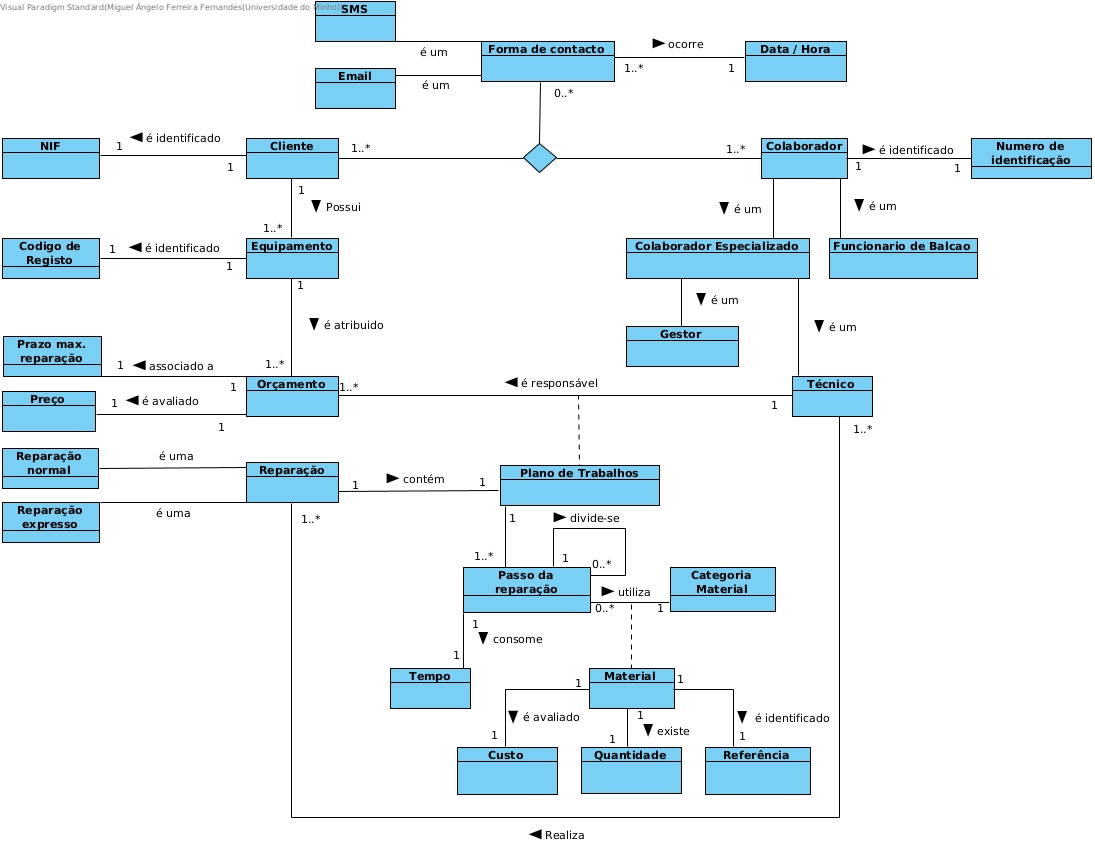
\includegraphics[scale=0.41]{Modelo.jpg}

\chapter{Modelação dos Requisitos Funcionais}
% O que o sistema deve fazer
Cenários foram identificados pela equipa docente.
% adicionar o diagrama de use case
A partir dos cenários foram identificados os seguintes \textit{use cases}:
\begin{itemize}
        \item Pedir orçamento - \ref{pedir_orcamento}
        \item Fazer orçamento - \ref{fazer_orcamento}
        \item Confirmar orçamento - \ref{confirmar_orcamento}
        \item Arquivar orçamento - \ref{arquivar_orcamento}
        \item Realizar reparação - \ref{realizar_rep}
        \item Entregar equipamento - \ref{entregar_equipamento}
        \item Pedir reparação expresso - \ref{pedir_rep_xpress}
        \item Registar equipamento - \ref{registar_equipamento}
        \item Registar cliente - \ref{registar_cliente}
        \item Listar resumida do técnico - \ref{listagem_tecnico_resumida}
        \item Listar detalhada do técnico - \ref{listagem_tecnico_detalhada}
        \item Listar funcionário do balcão - \ref{listagem_func_balcao}
\end{itemize}
\section{Modelo de Use Cases} % anexo ??

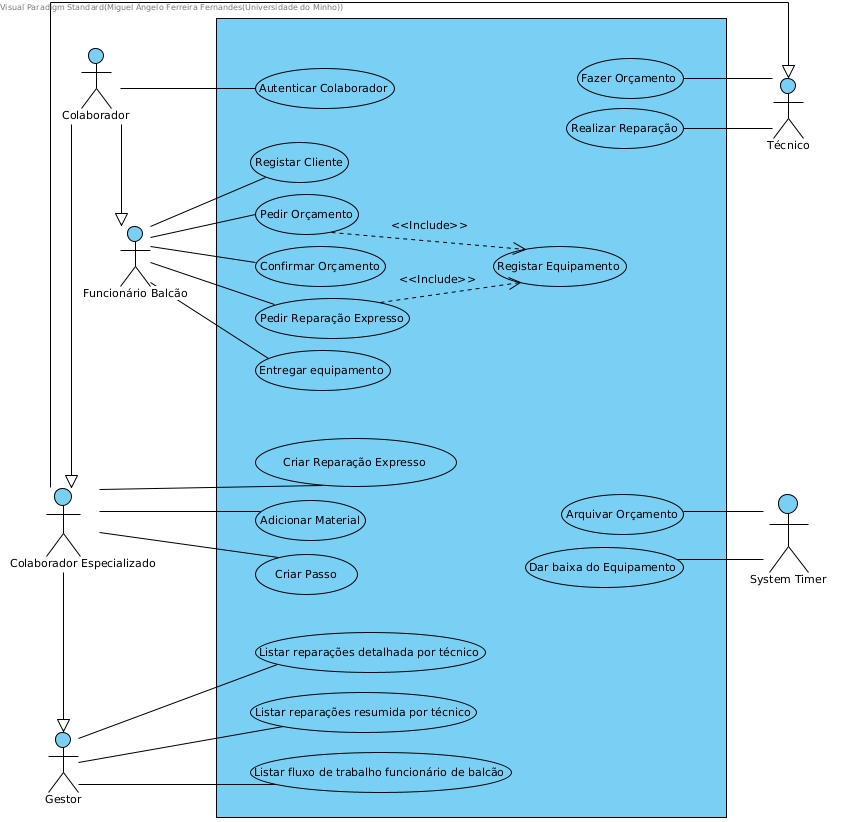
\includegraphics[scale=0.45]{dss-usecase.jpg}

\section{Especificação Use Cases}

\subsection{} \label{pedir_orcamento}
\subfile{use_cases/usecase_pedir-orcamento.tex}

\subsection{} \label{fazer_orcamento}
\subfile{use_cases/usecase_fazer-orcamento.tex}

\subsection{} \label{confirmar_orcamento}
\subfile{use_cases/usecase_confirmar-orcamento.tex}

\subsection{} \label{arquivar_orcamento}
\subfile{use_cases/usecase_arquivar-orcamento.tex}

\subsection{} \label{realizar_rep}
\subfile{use_cases/usecase_realizar-reparacao.tex}

\subsection{} \label{entregar_equipamento}
\subfile{use_cases/usecase_entregar-equipamento.tex}

\subsection{} \label{pedir_rep_xpress}
\subfile{use_cases/usecase_pedir-reparacao-expresso.tex}

\subsection{} \label{registar_equipamento}
\subfile{use_cases/usecase_registar-equipamento.tex}

\subsection{} \label{registar_cliente}
\subfile{use_cases/usecase_registar-cliente.tex}

\subsection{} \label{listagem_tecnico_resumida}
\subfile{use_cases/usecase_listar-tecnico-resumida.tex}

\subsection{} \label{listagem_tecnico_detalhada}
\subfile{use_cases/usecase_listar-tecnico-detalhada.tex}

\subsection{} \label{listagem_func_balcao}
\subfile{use_cases/usecase_listar-func-balcao.tex}

\chapter{Considerações Finais}
% análise crítica dos resultados

%==========================================================================
% BEGIN LISTA DE SIGLAS E ACRÓNIMOS
%==========================================================================

%% Portuguese babel does not translate this environment
\renewcommand{\nomname}{Lista de Siglas e Acrónimos}

%% Text that can be shown before acronyms list
\renewcommand{\nompreamble}{<<Apresentar uma lista com todas as siglas e acrónimos utilizados durante a realização do trabalho. O formato base para esta lista deverá ser da forma como abaixo se apresenta.>>}

%% acronyms
\nomenclature[01]{\textbf{BD}}{Base de Dados}
\nomenclature[02]{DW}{Data Warehouse}
\nomenclature[03]{OLTP}{On-Line Analytical Processing}
\nomenclature[04]{...}{...}

%% Show acronyms
\printnomenclature



%==========================================================================
% END LISTA DE SIGLAS E ACRÓNIMOS
%==========================================================================


%==========================================================================
% BEGIN ANEXOS
%==========================================================================

%% Why \addchap, instead of \chapter? 
%% \addchap has no numbering but appears in table of contents.
\addchap{Anexos}

    <<Os anexos deverão ser utilizados para a inclusão de informação adicional necessária para uma melhor compreensão do relatório o para complementar tópicos, secções ou assuntos abordados. Os anexos criados deverão ser numerados e possuir uma designação. Estes dados permitirão complementar o Índice geral do relatório relativamente à enumeração e apresentação dos diversos anexos.>>
    
    %% section version of \addchap
    \addsec{Anexo 1}


%==========================================================================
% END ANEXOS
%==========================================================================


\end{document}